\section{Experiments}\label{sec:set}

\begin{table*} %\small
  \centering
  \caption{Results on FB15k by relation category}
  \label{FB15k_results_by_relation_category}
  \begin{tabular}{c|cccc|cccc}
    \hline
    Task               & \multicolumn{4}{c|}{Predicting head(\textsc{Hits}@10(\%))} & \multicolumn{4}{c}{Predicting tail(\textsc{Hits}@10(\%))} \\
    \hline
    Relation Category  & 1-To-1        & 1-To-N        & N-To-1        & N-To-N        & 1-To-1        & 1-To-N        & N-To-1        & N-To-N \\
    \hline
%    SE                 & 35.6          & 62.6          & 17.2          & 37.5          & 34.9          & 14.6          & 68.3          & 41.3   \\
%    SME(linear)        & 35.1          & 53.7          & 19.0          & 40.3          & 32.7          & 14.9          & 61.6          & 43.3   \\
%    SME(bilinear)      & 30.9          & 69.6          & 19.9          & 38.6          & 28.2          & 13.1          & 76.0          & 41.8   \\
    TransE             & 43.7          & 65.7          & 18.2          & 47.2          & 43.7          & 19.7          & 66.7          & 50.0   \\
    TransH (unif)      & 66.7          & 81.7          & 30.2          & 57.4          & 63.7          & 30.1          & 83.2          & 60.8   \\
    TransH (bern)      & 66.8          & 87.6          & 28.7          & 64.5          & 65.5          & 39.8          & 83.3          & 67.2   \\
    TransR (unif)      & 76.9          & 77.9          & 38.1          & 66.9          & 76.2          & 38.4          & 76.2          & 69.1   \\
    TransR (bern)      & 78.8          & \textbf{89.2} & 34.1          & 69.2          & 79.2          & 37.4          & \textbf{90.4} & 72.1   \\
    CTransR (unif)     & 78.6          & 77.8          & 36.4          & 68.0          & 77.4          & 37.8          & 78.0          & 70.3   \\
    CTransR (bern)     & \textbf{81.5} & 89.0          & 34.7          & 71.2          & \textbf{80.8} & 38.6          & 90.1          & 73.8   \\
    \hline
    ATCE                & 71.0          & 60.3          & \textbf{83.9} & \textbf{81.9} & 70.3          & \textbf{89.9} & 76.0          & \textbf{89.2}   \\
    \hline
\end{tabular}
\end{table*}

\begin{table*} %\small
  \centering
  \caption{Results on FB15k-237 by relation category}
  \label{FB15k-237_results_by_relation_category}
  \begin{tabular}{c|cccc|cccc}
    \hline
    Task               & \multicolumn{4}{c|}{Predicting head(\textsc{Hits}@10(\%))} & \multicolumn{4}{c}{Predicting tail(\textsc{Hits}@10(\%))} \\
    \hline
    Relation Category  & 1-To-1        & 1-To-N        & N-To-1        & N-To-N        & 1-To-1        & 1-To-N        & N-To-1        & N-To-N \\
    \hline
%    SE                 & 35.6          & 62.6          & 17.2          & 37.5          & 34.9          & 14.6          & 68.3          & 41.3   \\
%    SME(linear)        & 35.1          & 53.7          & 19.0          & 40.3          & 32.7          & 14.9          & 61.6          & 43.3   \\
%    SME(bilinear)      & 30.9          & 69.6          & 19.9          & 38.6          & 28.2          & 13.1          & 76.0          & 41.8   \\
    TransE             & 43.7          & 65.7          & 18.2          & 47.2          & 43.7          & 19.7          & 66.7          & 50.0   \\
    TransH (unif)      & 66.7          & 81.7          & 30.2          & 57.4          & 63.7          & 30.1          & 83.2          & 60.8   \\
    TransH (bern)      & 66.8          & 87.6          & 28.7          & 64.5          & 65.5          & 39.8          & 83.3          & 67.2   \\
    TransR (unif)      & 76.9          & 77.9          & 38.1          & 66.9          & 76.2          & 38.4          & 76.2          & 69.1   \\
    TransR (bern)      & 78.8          & \textbf{89.2} & 34.1          & 69.2          & 79.2          & 37.4          & \textbf{90.4} & 72.1   \\
    CTransR (unif)     & 78.6          & 77.8          & 36.4          & 68.0          & 77.4          & 37.8          & 78.0          & 70.3   \\
    CTransR (bern)     & \textbf{81.5} & 89.0          & 34.7          & 71.2          & \textbf{80.8} & 38.6          & 90.1          & 73.8   \\
    \hline
    ATCE                & 71.0          & 60.3          & \textbf{83.9} & \textbf{81.9} & 70.3          & \textbf{89.9} & 76.0          & \textbf{89.2}   \\
    \hline
\end{tabular}
\end{table*}
\subsection{Experimental Setup}

\textbf{\indent Data Set.}
We use two widely-used benchmark data sets FB15k~\cite{BordesUGWY13} and FB15k-237 for evaluation, which are extracted from Freebase. FB15k has\fnum{592213} triples with\fnum{14951} entities and\fnum{1345} relationships.Triples in FB15k-237 are a subset of the FB15K set. FB15k-237 excludes redundant relations and direct training links for held-out triples, with the goal of making the task more realistic ~\cite{Toutanova15}.The two datasets are further divided into three parts for model training, tuning and evaluation. Specifically, we use FB15k and FB15k-237 since their triples are rich and closer to the real popular knowledge graph.

\textbf{Evaluation protocol.}
Following the same protocol used in \cite{BordesUGWY13}, we use \textit{Mean Rank} and \textit{Hits@10} as evaluation protocals of our model. For each test triple $(h,r,t)$, we replace tail head $t$(or the head $h$) with each entity $e$ in $\mathcal{E}$ to generate \emph{corrupted triples} and calculate the scores of each triple using the score function. After ranking the scores in descending order, we then get the rank of the correct entity. \textit{Mean Rank} is the mean of all the predicted ranks, and \textit{Hits@10} denotes the proportion of correct entities ranked in the top 10. Note that, a corrupted triple ranking above a test triple could be valid, which should not be counted as an error. To eliminate the effects of such condition, corrupted triples that already exist in the KG are filtered before ranking. In this case, the setting of evaluation is called "Filter", while the original one is called "Raw". Since this effect ,the "Filter" setting is more preferred. In both settings, a higher Hits@10 imply the better performance of a model.

\textbf{Baselines.}
We use a few outstanding models in recent years as baselines and compare our model with them, including TransE~\cite{BordesUGWY13}, TransH~\cite{WangZFC14}, TransR~\cite{LinLSLZ15} , CTransR~\cite{LinLSLZ15}, PTransE~\cite{LinLLSRL15} and GAKE~\cite{FengHYZ16}. For each baseline model, we first learn representations of all entities and relations. After that the conditional probability of a triple is calculated by the score function, While in ATCE, we construct the triple context with each triple. At last, if the conditional probability of $<h,r,t>$ is larger than $p_r$,  $<h,r,t>$ is regard as a correct triple.

\begin{table} %\small
  \caption{Link prediction results}
  \label{table_link_prediction_results}
  \begin{tabular}{c|cc|cc}
    \hline
    \multirow{2}{*}{Metric}  & \multicolumn{2}{c|}{Mean Rank} & \multicolumn{2}{c}{\textsc{Hits}@10(\%)} \\
                             & Raw          & Filter          & Raw           & Filter          \\
    \hline
%    RESCAL                   & 828          & 683             & 28.4          & 44.1            \\
%    SE                       & 273          & 162             & 28.8          & 39.8            \\
%    SME(linear)              & 274          & 154             & 30.7          & 40.8            \\
%    SME(bilinear)            & 284          & 158             & 31.3          & 41.3            \\
%    LFM                      & 283          & 164             & 26.0          & 33.1            \\
    TransE                   & 243          & 125             & 34.9          & 47.1            \\
    TransH (unif)            & 211          & 84              & 42.5          & 58.5            \\
    TransH (bern)            & 212          & 87              & 45.7          & 64.4            \\
    TransR (unif)            & 226          & 78              & 43.8          & 65.5            \\
    TransR (bern)            & 198          & 77              & 48.2          & 68.7            \\
    CTransR (unif)           & 233          & 82              & 44.0          & 66.3            \\
    CTransR (bern)           & 199          & 75              & 48.4          & 70.2            \\
    PTransE                  & 207          & 58              & 51.4          & \textbf{84.6}   \\
    GAKE                     & 228          & 119             & 44.5          & 64.8            \\
    \hline
    ATCE                      & \textbf{110} & \textbf{25}     & \textbf{55.3} & 83.1            \\
    \hline
  \end{tabular}
\end{table}

\textbf{Implementation.}
We construct the knowledge graph using Apache TinkerPop\footnote{\url{http://tinkerpop.apache.org/}}, an open source graph computing framework. In a few cases, the reverse relation, an edge labeled $r^{-1}$ from $t$ to $h$ for the triple $(h,r,t)$, would be useful when representing some patterns in the graph. For instance, the relation path $a \xrightarrow{motherOf} b \xleftarrow{fatherOf} c$, i.e., $(a, motherOf, b)$ and $(c, fatherOf, b)$, indicates a potential relation $marriedTo$ between $a$ and $c$. Therefore, we add reverse relation of each relation into KG. Specifically, for each edge labeled $r$ from $h$ to $t$ in the graph, we add another edge labeled $r^{-1}$ from $t$ to $h$.

For neighbor context generation, it's expensive to consider all the neighbors of each entity in the graph for the reason that there are some entities connecting with a large amount of other entities, which would lead to a huge size of neighbor context. We use sampling to reduce the size of neighbor context. For those entity whose neighbor context size is larger than a fixed size $n$, we sample $n$ neighbors randomly from it's neighbor context. Similarly, a large number of paths between a pair of entities would result in high computational complexity. To solve the problem, firstly, we limit the length of paths by 2-step and 3-step, then, we use random walk to sample $m$ paths between a pair of entities. In our experiment, $n$ and $m$ are all set as 10. Note that for some pairs of entities, there may be no 2 or 3 step relation paths. In such case, we suppose that the relatedness between those pairs of entities are relatively low and the values of $g_P(\cdot, \cdot)$ in Eq.~\eqref{gp} are set as -100. We store all triple contexts in Mongodb\footnote{\url{www.mongodb.org/}},a NoSQL database, that can help us for rapid seeking the context of a specified entity.


We use mini-batch SGD to train our model. We choose the learning rate $\alpha$ of SGD among $\{0.1, 0.01, 0.001\}$, the dimension of embeddings $k$ among $\{50, 75, 100\}$, the batch size $B$ among $\{120, 480,$ $ 960, 1920, 4800\}$. The best parameters are determined by the performance on valid set. The optimal parameters are $\alpha=0.001$, $k=50$ and $B=4800$.

\subsection{Link Prediction}
Link prediction~\cite{BordesUGWY13} is a task to predict the missing head or tail entity in a given triple based on training triples. Metrics \textit{Mean Rank} and \textit{Hits@10} are used to measure the performance of our model.


We collected the result of link prediction in Table~\ref{table_link_prediction_results}. From the results we can see that, our model outperforms other baselines on most of the metrics significantly and consistently, while slightly worse than PTransE on \textsc{Hits}@10. The result implies that triple contexts do improve the performance on link prediction. Although using similar types of contexts in the graph, GAKE's performance is inferior to our model, which shows the superiority of our framework. Note that the experimental results of \textsc{HolE} are absent here, for it uses a different metric, MRR (Mean Reciprocal rank), instead of \textit{Mean rank} for evaluation. But according to \textit{Hits@10} reported in~\cite{NickelRP16}, the results of our model are better than \textsc{HolE}.


In Table~\ref{FB15k_results_by_relation_category} and Table~\ref{FB15k-237_results_by_relation_category}, we show separate evaluation results by category of relationships on FB15k. We can see that ATCE brings promising improvements on modeling complex relations, such as predicting tail of 1-To-N relations, predicting head of N-To-1 relations and N-To-N relations. Specifically, ATCE behaves well when predicting the "N" side of 1-To-N and N-To-1 relations, indicating that valid triples have higher scores than invalid triples in general. In some other simpler scenarios, such as 1-To-1 relations and predicting the "1" side of 1-To-N and N-To-1 relations, the performance of ATCE is still acceptable although not so good as some other baselines, such as TransH and TransR. The results suggest that the incorporation of triple context is helpful when handling complex relations, at the cost of precision in modeling simple relations, which seems complementary to some other baselines.
\subsection{Triple Classification}
We also test our model on triple classification. In this task,given a knowledge base and a triple $<h,r,t>$ we aim to determine whether it is correct or not. FB15K has only positive examples, thus we generated negative triples for FB15K by following strategy of ~\cite{socher2013}. As the result, the classification accuracies on FB15K and FB15k-237 can be compare directly with previous studies. In this task, we choose TransE,TransH,TransR,TransD,NTN and GAKE as baseline models. The parameter values for training TransE,TransH,TransR,TransD,NTN and GAKE are borrowed from their reports.

\begin{table}
 \centering
 \caption{Triple Classification results}
  \label{Triple Classification_results}
\begin{tabular}{c|c|c}
  \hline
  Start & FB15k  & FB15k-237 \\
  \hline
  TransE & 0.81 & 0.82 \\
  TransH & 0.81 & 0.81 \\
  TransR & 0.82 & 0.82 \\
  TransD & 0.87 & 0.87 \\
  GAKE & 0.89 & 0.88 \\
  NTN & 0.41 & 0.42 \\
  \hline
  ATCR & \textbf{0.91} & \textbf{0.92} \\
  \hline
\end{tabular}
\end{table}
In Table ~\ref{Triple Classification_results}, we shows the accuracies of triple classification on two datasets. The context preserving embeddings in general outperform their base model. As the table shows, ATCE always has higher accuracy than TransE,TransH,TransR,TransD,NTN and GAKE. One thing to note is that the improvements by the context preserving embeddings are always observed in FB15k, while those in FB15-237 are small or slightly negative. This can be explained with number of triples with a transitive or symmetric relation in the dataset. In FB15k-237, this kinds of triples are removed from FB15k. Thus the improvement in FB15K is remarkable, our approach outperforms others by 11.04\% in terms of accuracy on average as the triple context brings more information especially relations between entities when learning the knowledge graph representations.

Furthermore, to better understand the attention mechanism in our approach, The examples of path are selected by attention mechanism in path context are shown in Table ~\ref{Attention Results in Path Context}. The number in front each line is the weight score, which is computed by the attention mechanism for each relation. From the examples we can see that ATCE successfully combines structure learning and parameter learning. It not only choose multiple connective path between two entities to capture the complex structure in the knowledge base, but also learn weight score of the path for a specific relation.

\begin{table}
 \centering
 \caption{Attention Results in Path Context}
  \label{Attention Results in Path Context}
  \small
  \setlength{\tabcolsep}{1mm}{
\begin{tabular}{c|l|l}
  \hline
  Weight & Path  & Relation \\
  \hline
  0.45 &  $contains \xrightarrow{} contains $ & $partially\_contains$ \\
  0.35 & $contains \xrightarrow{} nationality$ & $marriage\_location$ \\
  0.24 & $nationality$ & $marriage\_location$ \\
  0.35 & $contains \xrightarrow{} place\_lived$ & $marriage\_location$ \\
  0.2 & $nominated\_for$ & $film\_edited\_by$\\
  0.3 & $nominated \xrightarrow{} award\_nominee$ & $film\_edited\_by$\\
  \hline
\end{tabular}}
\end{table}

For neighbor context, we also use attention mechanism to choose which neighbor is more related for the head. we demonstrate attentions of the 6 different neighbors when they are regards as the neighbor context of the entity $Terminate2:JudgementDay$, which indicates a movie in 1991. Figure ~\ref{pic2}  shows the results, from the results we see two entities, $Action$ and $Sequel$ ,have largest attention to represent the target entity $Terminate2:JudgementDay$, as $Action$  reflects the type of movie while only some of movies have sequels.
\begin{figure}
  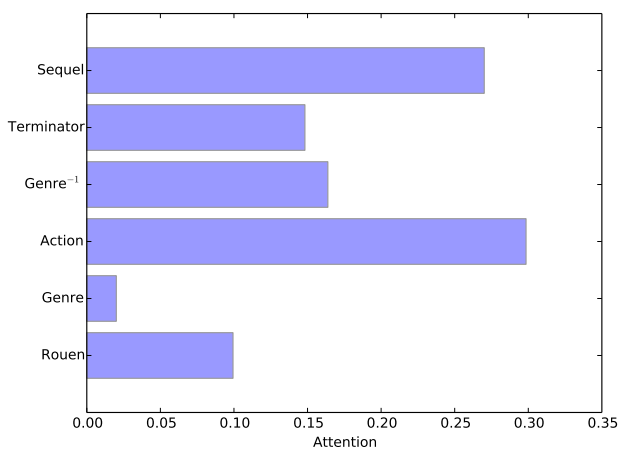
\includegraphics[width=0.45\textwidth]{pic2.png}
  \caption{Attentions for neighbor context of  \emph{Terminate2:JudgementDay}}
  \label{pic2}
\end{figure}








